\documentclass[oneside]{article}
\setlength{\oddsidemargin}{0.25 in}
\setlength{\evensidemargin}{-0.25 in}
\setlength{\topmargin}{-0.6 in}
\setlength{\textwidth}{6.5 in}
\setlength{\textheight}{8.5 in}
\setlength{\headsep}{0.75 in}
\setlength{\parindent}{0 in}
\setlength{\parskip}{0.1 in}
\setcounter{section}{0}
\setcounter{subsection}{-1}
%
% ADD PACKAGES here:
\usepackage{float}
\usepackage{pdfpages}
\usepackage{graphicx}
\usepackage{amsmath,amsfonts,amssymb,graphicx,mathtools,flexisym, hyperref, graphicx}
\usepackage{amsmath,systeme}
\usepackage{tcolorbox}
\usepackage{enumerate}
\usepackage{tikz}
\usepackage{listings}
\usepackage{xcolor}
\usepackage{bm}
\usepackage{lipsum}
\usepackage{amsmath}
\usepackage{amsthm}
\usepackage{acronym}
\usepackage{algpseudocode}
\usepackage{algorithm}
\usepackage{fancyvrb}
%\usepackage{biblatex} %Imports biblatex package
%\addbibresource{reference.bib} %Import the bibliography file
\definecolor{commentgreen}{RGB}{2,112,10}
\definecolor{eminence}{RGB}{108,48,130}
\definecolor{weborange}{RGB}{255,165,0}
\definecolor{frenchplum}{RGB}{129,20,83}


\definecolor{codegreen}{rgb}{0,0.6,0}
\definecolor{codegray}{rgb}{0.5,0.5,0.5}
\definecolor{codepurple}{rgb}{0.58,0,0.82}
\definecolor{backcolour}{rgb}{0.95,0.95,0.92}
\newcommand{\E}{\mathbb{E}}
\newcommand{\V}{\mathbb{V}}
\renewcommand{\P}{\text{I\kern-0.15em P}}


\tcbuselibrary{theorems}
\newtcbtheorem
  []% init options
  {theorem_exam}% name
  {Theorem}% title
  {%
    colback=orange!5,
    colframe=orange!35!black,
    fonttitle=\bfseries,
  }% options
  {def}% prefix


\newtcbtheorem
  []% init options
  {definition_exam}% name
  {Definition}% title
  {%
    colback=blue!5,
    colframe=blue!35!black,
    fonttitle=\bfseries,
  }% options
  {def}% prefix  


\newtcbtheorem
  []% init options
  {proposition_exam}% name
  {Proposition}% title
  {%
    colback=red!5,
    colframe=red!35!black,
    fonttitle=\bfseries,
  }% options
  {def}% prefix  

\newcommand{\Lim}[1]{\raisebox{0.5ex}{\scalebox{0.8}{$\displaystyle \lim_{#1}\;$}}}
\newcommand{\Inf}[1]{\raisebox{0.5ex}{\scalebox{0.8}{$\displaystyle \inf_{#1}\;$}}}
\newcommand{\Sup}[1]{\raisebox{0.5ex}{\scalebox{0.8}{$\displaystyle \sup_{#1}\;$}}}
\newcommand{\norm}[1]{\left\lVert#1\right\rVert}
%
% To generate a clickable table of content.
%
\hypersetup{
    colorlinks,
    citecolor=black,
    filecolor=black,
    linkcolor=black,
    urlcolor=blue
}


\algdef{SE}{Begin}{End}{\textbf{begin}}{\textbf{end}}


\usepackage{tocloft}

\addtolength{\cftsecnumwidth}{10pt}
\setlength{\cftsubsecnumwidth}{3.5em}
\usepackage[utf8]{inputenc}

% Default fixed font does not support bold face
\DeclareFixedFont{\ttb}{T1}{txtt}{bx}{n}{12} % for bold
\DeclareFixedFont{\ttm}{T1}{txtt}{m}{n}{12}  % for normal

% Custom colors
\usepackage{color}
\definecolor{deepblue}{rgb}{0,0,0.5}
\definecolor{deepred}{rgb}{0.6,0,0}
\definecolor{deepgreen}{rgb}{0,0.5,0}

\usepackage{listings}

% Python style for highlighting
\newcommand\pythonstyle{\lstset{
language=Python,
basicstyle=\ttm,
morekeywords={self},              % Add keywords here
keywordstyle=\ttb\color{deepblue},
emph={MyClass,__init__},          % Custom highlighting
emphstyle=\ttb\color{deepred},    % Custom highlighting style
stringstyle=\color{deepgreen},
frame=tb,                         % Any extra options here
showstringspaces=false
}}


% Python environment
\lstnewenvironment{python}[1][]
{
\pythonstyle
\lstset{#1}
}
{}

% Python for external files
\newcommand\pythonexternal[2][]{{
\pythonstyle
\lstinputlisting[#1]{#2}}}

% Python for inline
\newcommand\pythoninline[1]{{\pythonstyle\lstinline!#1!}}



\title{Brain 5}
\date{S1 2022}


\begin{document}

\pagenumbering{gobble}
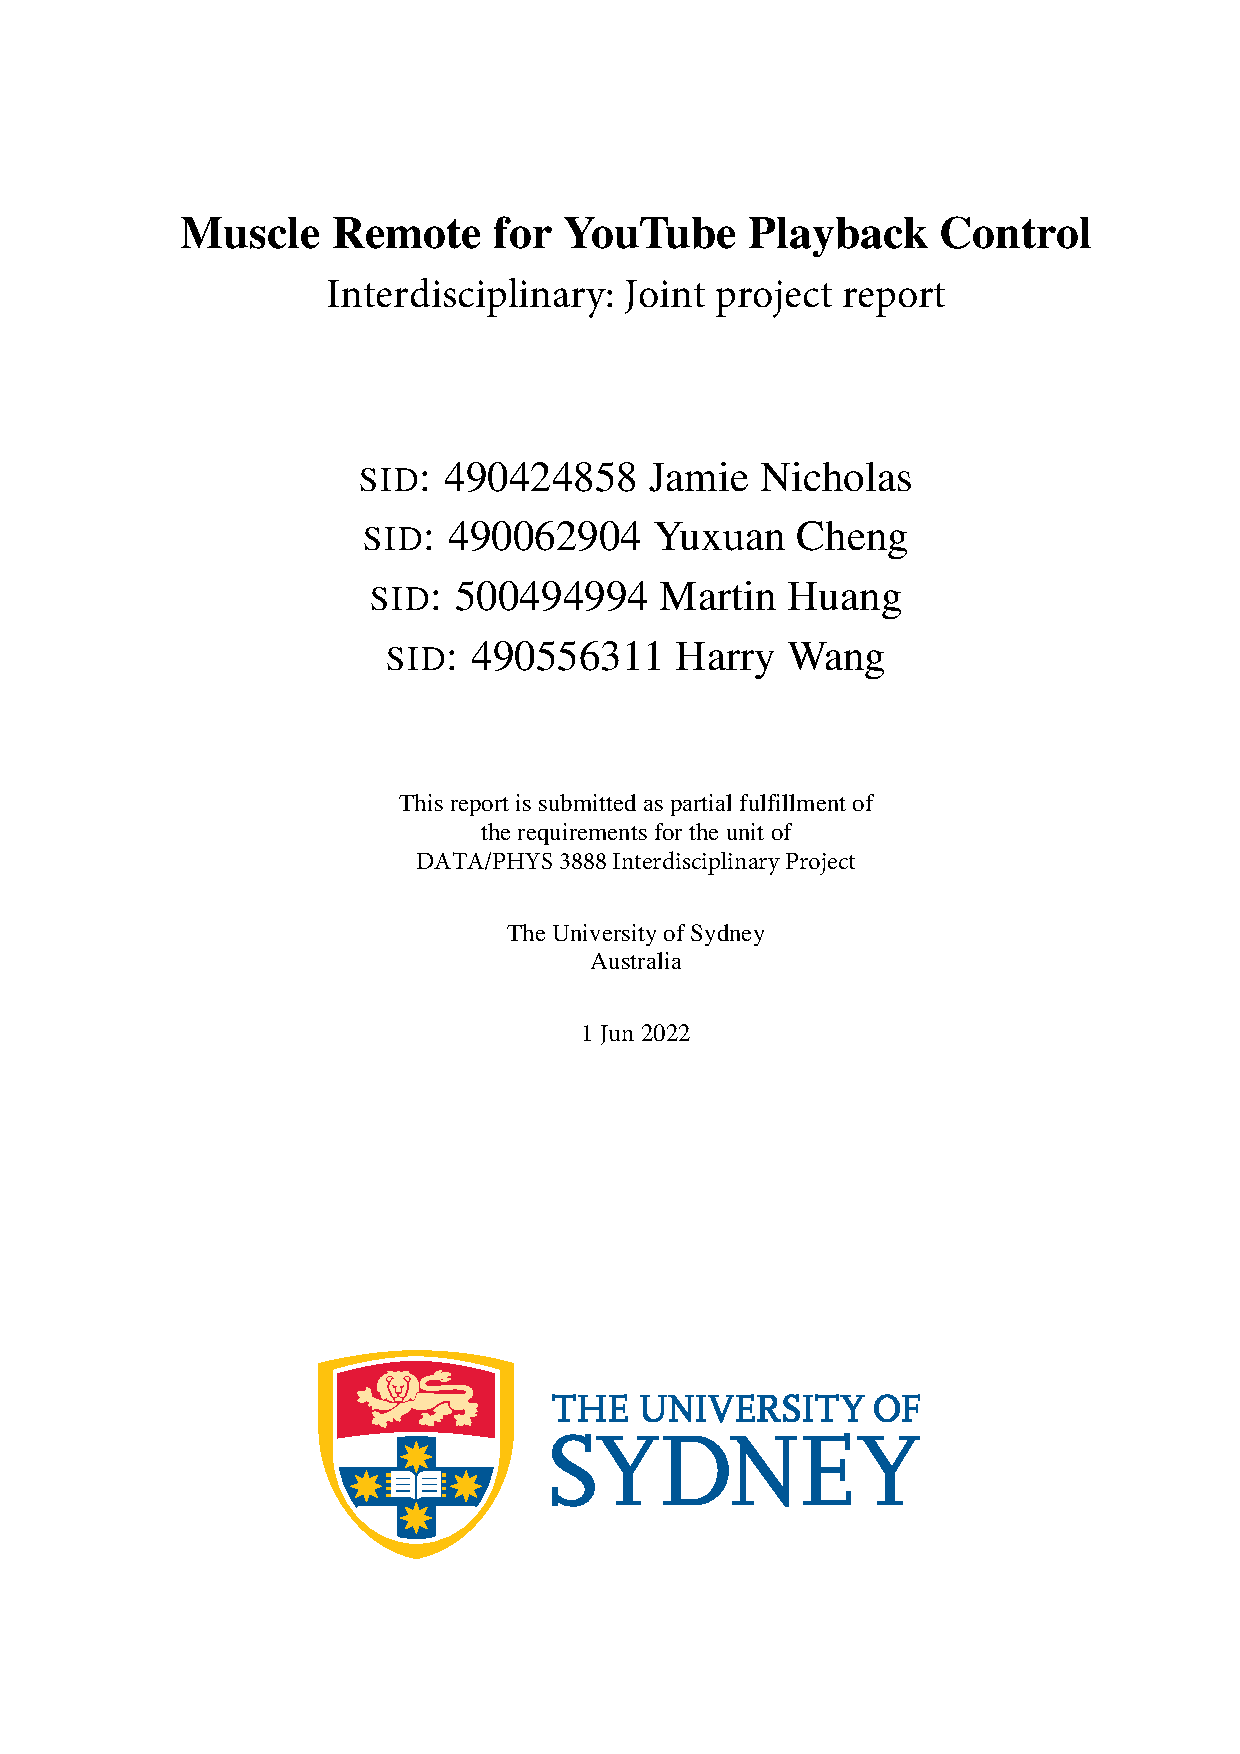
\includepdf[pages=-]{title_page.pdf}

\newpage
\tableofcontents
\newpage
\pagenumbering{arabic}


\section{Executive Summary}
In this report, we detail the process of creating a muscle remote for YouTube playback control. Given the current rate of technological progression and the increasing user time spent using such technology it is crucial that all members of society are able to participate/use such advancements. Specifically, people with limited finger dexterity; preventing them from using technology in a traditional means.This includes people with disabilities, gamers looking for an  alternate style of controller and professionals or students doing presentations. As such we want to create a device that allows our target audience to participate in technology use including our YouTube playback control and any future developments towards a universal open source product. 

During the development process, we found key insights into the success and direction of our final product. By utilising electrodes and a 'SpikerBox’ we were able to create the YouTube media remote through changes in voltage from the electrodes. Various sequences of the arm movements create different patterns of voltage and frequency. It is important to note however that the product is susceptible to external variables through noise. This includes making small changes in the placement of the electrodes. Accordingly, any classifier created needed to accommodate for variations in the voltage as a result of these inconsistencies. 

Our workflow is as follows: 


\begin{figure}[H]
  \centering
  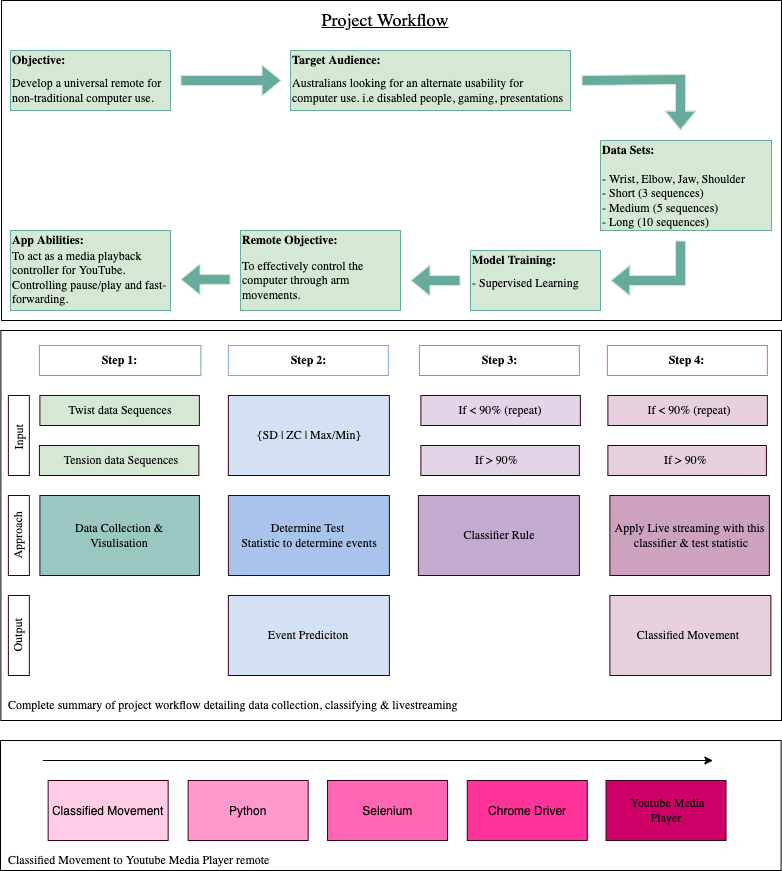
\includegraphics[width=11cm]{Pictures/1.png}
  \caption{Project Workflow}
  \end{figure}

\section{Background, Motivation and Aim}
As technology's rapid growth has led to the everyday consumer becoming increasingly reliant on it for everyday tasks, there comes a need for a greater variety of tools to interact with such technology in a more efficient manner. Effectively looking to increase the usability for user convenience. Intuitively, for our product this involves a scenario where a user may be watching Netflix’s and rather than using a remote to watch the next episode they can twist their arm to trigger the action. This removes the need for hard copy style tv remote. 

Investigation into the current market for gesture-based media systems shows that there has been progress in the field however often the system is brand specific meaning that the gestures can’t be transferred between platforms. Our remote hopes to be usable across multiple different platforms. Moreover, from the products that do exist many require the use of a large external ‘remote style’ device; something which we hope to remove. The two electrode system is an effective starting point for creating a user-friendly gesture system. 


\section{Methods and Results}
The apparatus used during the development of our product includes the stand-alone neuron ‘SpikerBox’ a product of Backyard Brains which is a bio-amplifier translating electrical signals from neurons and  muscles. 

\subsection{Electrode Placement}
Three electrodes are required to make the needed measurements; 2 to measure the signal and 1 to act as the ground. Part of the testing phase included finding positions that produced the strongest signal with the least background noise. We conducted tests over various points of the forearm, shoulder, wrist, elbow and jaw. At each body part a series of data was collected. Including a short(3 sequence event), medium (5 sequence event) and long(10 sequence event) sequence of movements across 3 separate individuals. We found body parts with high muscular contraction producing the best signal, that being the top point of the forearm. With regard to the ground we found that with the movement of the elbow it was not working effectively, so we adjusted the ground to the initial position on the back of the jaw. This provided the least background noise. It is worth noting that the same data could be used to test the accuracy of the classifier later. 

\subsection{Spiker Recordings Findings}
\label{spikefind}
It is possible to assign different commands to the permutations of one arm movement, while this brings unnecessary difficulties in movements classification. Instead, we designed two arm movements with distinct frequency spectrum. In particular, arm twisting and arm tension, they both have electric signal over the frequency range from 10Hz to 100 Hz. 
\begin{figure}[H]
  \centering
  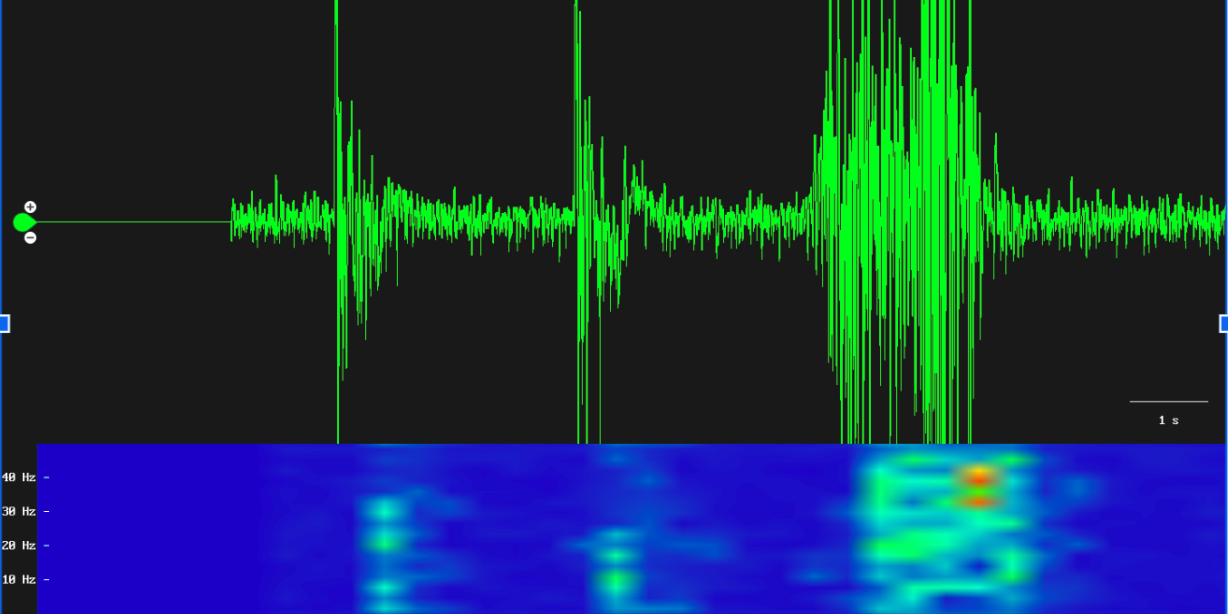
\includegraphics[width = 17cm, height = 3.5cm]{Pictures/UUE_1.png}
  \caption{The electric signal and frequency spectrum of two twisting and one tension in order from SpikeRecorder.(notch filter at 50Hz applied)}
  \label{UUE1}
  \end{figure}
As presented in the Figure \ref{UUE1}, the arm tension displayed intense signal over the range of 30Hz to 50Hz, while the signal from arm twisting has relatively mild signals that are evenly distributed over the whole range.
\newline
\newline
However, There is no characteristic frequency of these two movements. The frequency spectrum depends on different person with their different ways of twisting and tensing their arm. This frequency spectrum differs between various group members.
%Figure \ref{UUE2} is the frequency spectrum from another group member.  
%\begin{figure}[H]
%  \centering
%  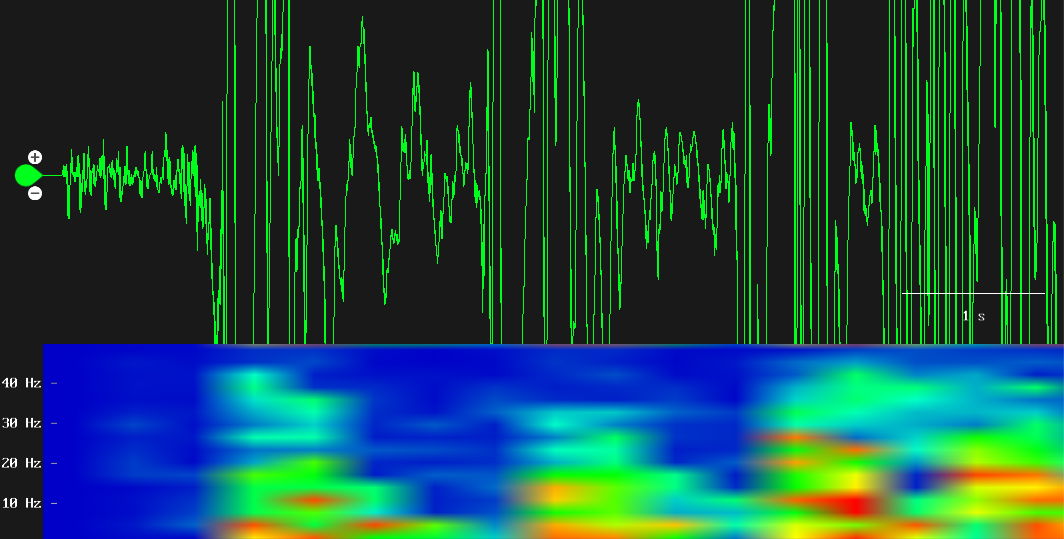
\includegraphics[width = 8cm, height = 3.5cm]{Pictures/UUE_2.png}
%  \caption{The electric signal and frequency spectrum of two %twisting and one tension in order,from another group member.(notch %filter at 50Hz applied)}
%  \label{UUE2}
%\end{figure}
 Arm twisting has an intense signal over low range frequency. Hence, it will be inaccurate to classify two movements by frequency and the corresponding intensity of signal as the intensity varies between users. We can observe that the frequency spectrum for twisting and tension maintains the pattern that only tension has intense signal over higher frequency range,thus there is a notable distinction in the duration of two movements. This proved to be helpful in designing the classifier.
\subsection{Filtering and Streaming Decisions}
In order to identify predicted event intervals more easily, we first attempted to use low level filtering, this included downsampling of only every 100 data entries. We then used standard deviation to determine predicted intervals. From this we found that the predicted intervals did in fact include the events, however would be much longer than the event and include white noise. Because of this, we decide to use Inverse Fast Fourier Transformation (IFFT) to produce a filtered wave, with less white noise. 



\subsection{Feature Extraction}
Using the filtered signal, we use standard deviation as our test statistic in order to predict interval events through each window. Utilising a threshold event of 12, meaning that for all standard deviations calculated, if it is greater than 12, we identify it as a possible event. 

From here, we must consider 2 configurations for our feature extraction and classifier choice. Firstly, our function as it has small windows always predicts more intervals than actual events. In order to predict the same number of events, we combine intervals if they are within a certain distance of each other (in regard to time). For example if we made this predetermined distance as 1 second, Intervals such as (0,0.5) and (0.7,1.3) would be combined together, as we see that the distance between the end of the first event and start of the second event is less than 1. Therefore, our new interval will be (0,1.3). Secondly, in our classifier, we need to find a difference value for when we think the user tenses their arm, or turns it. 

For example, if we find our predicted interval (say the same as above) of (0,1.3), if we stated that all intervals less than 1 second is classified as a tension, and all intervals greater than 1 is a turn. So in this case, 1.3-0 = 1.3, therefore classify this as a non-tension. In python, we tested 400 different configurations of distance of intervals, and also difference of intervals in order to choose the optimal classifier and predicted interval. These 400 configurations came from values 0 to 2 with 0.1 increments for both two configurations. Upon inspection, we saw that there were no significant accuracy values between 0 - 0.5, therefore we decide to start from 0.5 for the difference value and take 0.05 increments, thus we now have 0.5 to 2 values with increments 0.05 for the difference configuration, and 0 - 2 values with increments 0.1 for the interval configurations, giving us 672 total unique configurations. From this we found the maximum accuracy of 0.809 which came from an interval value of 1.1 and Difference value of 1.25. The spread of the accuracies can be found below, from 672 tests. See appendix 1 for code. Testing it with the three types of wave files short medium and long: 
 
\begin{figure}[H]
  \centering
  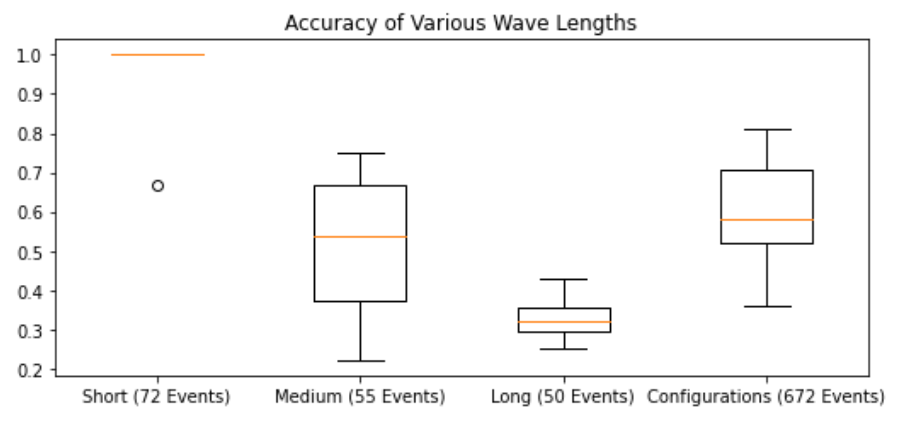
\includegraphics[width=12cm]{Pictures/accuracytt.png}
  \caption{Accuracy of Training Data and Configurations for Unique Modified Classification Rule}
 
  \end{figure}
  

\subsection{Classifier Choice}

Based on the multiple tests conducted above, we decide to go with the optimal configuration and decide that intervals of less than 1.25 are considered an event of Tension, whilst intervals greater than 1.25 are regarded as Turns. This provided 81\% accuracy from 114 events.

Let $E$ be an array such that $|E| = 2$
$$
\text{Event is} 
    \begin{cases} 
       \text{Tension}; & E[1] - E[0] \leq 1.25\\
       \text{Turn}; & E[1] - E[0] > 1.25
    \end{cases}
$$
\subsubsection{Limitations of Classifier}

We also had 4 files, with "errors" in them, meaning that there is no obvious event. For example, we had a stable wave, which is a wave with no intended movements. For this, our classifier actually was correct and did not produce any output. The next error file, we had random movements in the arm, which the classifier predicted 2 tension movements. Obviously this is not correct. Finally, we had the user conduct a stretch of their arms, which our classifier thought there were 2 tension movements. Looking forward, our product could implement a no movement or error detection in order to not incorrectly predict events.  

In addition to this, we found that user who has more hair than some other users may have a lower accuracy in the classifier. This is due to the electrode not being able to record the data as clearly, as there is some hair interfering. 


\subsection{Live Classifier} 

During the deployment stage of our classifier, we have exhibited major performance losses. We suspect the cause to mainly associate with the filter we use. Since in live streaming condition there will only be cached data from the past but not the future, Fourier transformation will not function the same as on the recorded data.

We used live testing on 4 different subjects, recording data and accuracy of short wave files (3 events each), medium wave files (5 events each) and long wave files (10 events each). The accuracy spread and box-plot can be seen. This demonstrates the limitation of the live classifier for different users. One way to standardise user accuracy, is by including a set of instructions for what is actually considered tension and turn. For example, for tension, we must need the user to tense with the focus on the forearm, rather than the bicep and/or triceps. In addition to this, for turning, we expect a sharp turn lasting only around 1 second long, rather than a slow continuous turn. While informing the user of these instructions, we would see a more standardised and similar result on each individual. 

In this test, we had all users sitting down, as this is what the product is intended for. In addition to this, we had the exact same electrode placement for each individual, which was already decided in section 3.1. Each user was told what sequence of events to record, and an accuracy was manually recorded.

\begin{figure}[H]
  \centering
  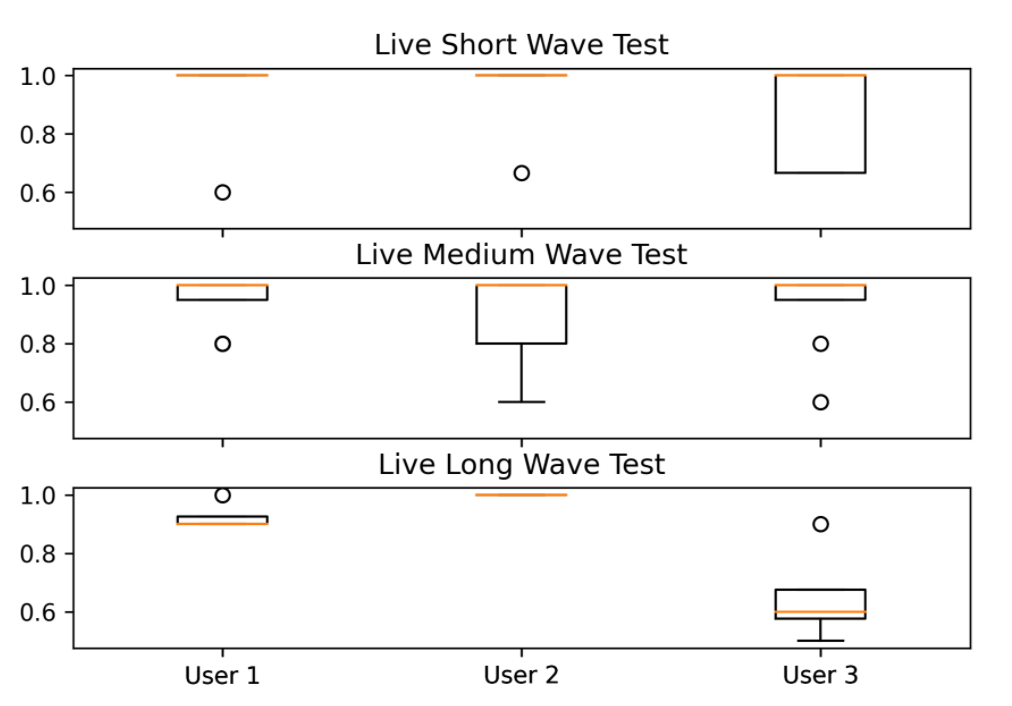
\includegraphics[width = 10cm]{Pictures/livetest.png}
  \caption{Accuracy Comparison for Live Testing on Three Separate Users}
  \end{figure}


\subsection{Deployment}
With an modified classifier that perform generally well under live-streaming condition, the next step would be deploying it to perform YouTube media player playback control.
The main package that would be used in deployment is Selenium. Selenium provides us the ability to automate browser interaction directly from Python.  
We have included the web driver chrome version 102 for m1 mac in our code-base, user of other systems and chrome version should download a corresponding web driver for their system from https://chromedriver.chromium.org/downloads.

After a YouTube video page have been loaded Selenium will grab the media player element and assign it to an variable "video".
Whenever the live classifier detects a twist or turn of the forearm, the script will simulate a keyboard "SPACE" and send to the video element to toggle play/pause of the video. Similarly, when tension is detected, the script will simulate a "ARROW\_RIGHT" key press to trigger a fast forward of five seconds.




\section{Discussion}
In section \ref{spikefind}, we see that the arm tension and arm twisting have different pattern of frequency spectrum. Those signals are from the skeletal muscles on forearm. The skeletal muscles generate electric signals, which corresponds to the change in electric potential, by the combination of isotonic contraction (shorten the length of muscles) and isometric contraction (without shortening the length). In having hand and arm movements, the flexor digitorum superficialis are measured to give the strongest signals \cite{muscleResponse} (the flexor digitorum superficialis is the deep layer arm muscles under the  brachioradialis muscles, see the configuration in Figure \ref{arm}).
\begin{figure}[H]
  \centering
  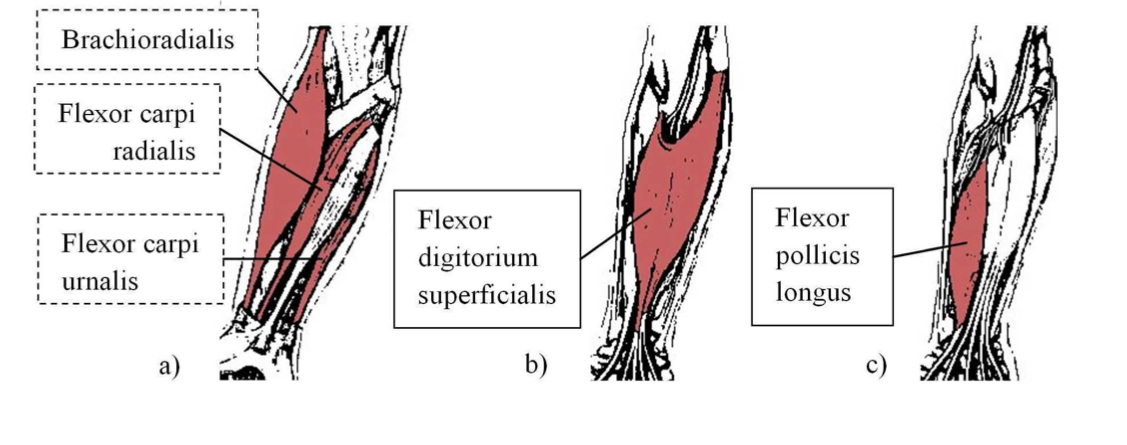
\includegraphics[width = 8cm, height = 3.5cm]{Pictures/armMuscle.png}
  \caption{The forearm muscles configuration, cite from \cite{muscleResponse}}
  \label{arm}
\end{figure}
When the arm is twisted, this part of muscle is not activated since the strongest movement happens in wrist. Arm tension however is a direct movement of flexor digitorum superficialis. This leads to the weak intensity of electric signal in arm twisting compared with arm tension. Moreover, there is no significant statistical difference for the positions of electrodes on forearm \cite{muscleResponse}. We confirmed this by changing electrodes configurations from opposites side of arm to parallel side and obtained the same pattern of frequency spectrum.


\section{Limitations of the Product}

There are two main limitations regarding our product. Firstly, the program is made such that the consumer must follow a set of instructions, in order for the product to correctly estimate arm movements. For example, the tension of arms is not estimated based on the amount of energy you exert while tensing, but rather the length of how long you tense. This is extended into turning. The consumer should have a short and fast supination action in order for optimal accuracy. In order to combat this, for our product we can include an instruction manual and also a YouTube video, showing a visual example on how to maximise accuracy.

Our second main limitation is the recording of waves, based on the interference between electrodes and skin. Users with a greater volume of hair on their arms may experience a lower accuracy than users with smoother arms, due to the interference. As waves produce more white noise, the accuracy is lower as well. Another concern is that our third electrode is situated at the back of the jaw. This is not an ideal location as it could potentially be in the way of the user, and is not discrete. In the future, we can test for better electrode placement which makes it easier for the consumer, such as somewhere along the wrist, if we were planning to implement it for smart watch compatibility. 

\section{Conclusion}
Critical to the success of our muscle remote for YouTube playback control was communication and effective teamwork. By carefully curating our workflow and managing time we were able to collect data via spikerboxes to create sequences of wave functions. Once classified using a standard deviation method the data was then able to control Youtube. Future work could include looking into how to make the remote universal to other media playback programs such as Netflix or Spotify. Additionally, implementation into smart watches would be ergonomic progress for the remote. 
\newpage
\section{Appendix}

Please note that all code generated graphs and python scripts can be found on the Github Repository found in  \href{https://github.com/yingzhenwang/Brain}{here}. Figure 3 and 4 can both be found in \href{https://github.com/yingzhenwang/Brain/blob/main/notebook.ipynb}{notebook.ipynb}


\subsection{Part 1: Arduino Data Recorder}

Code can be found in  \href{https://github.com/yingzhenwang/Brain/blob/main/Chrome/live.py}{live.py}

\begin{figure}[H]
 \centering
  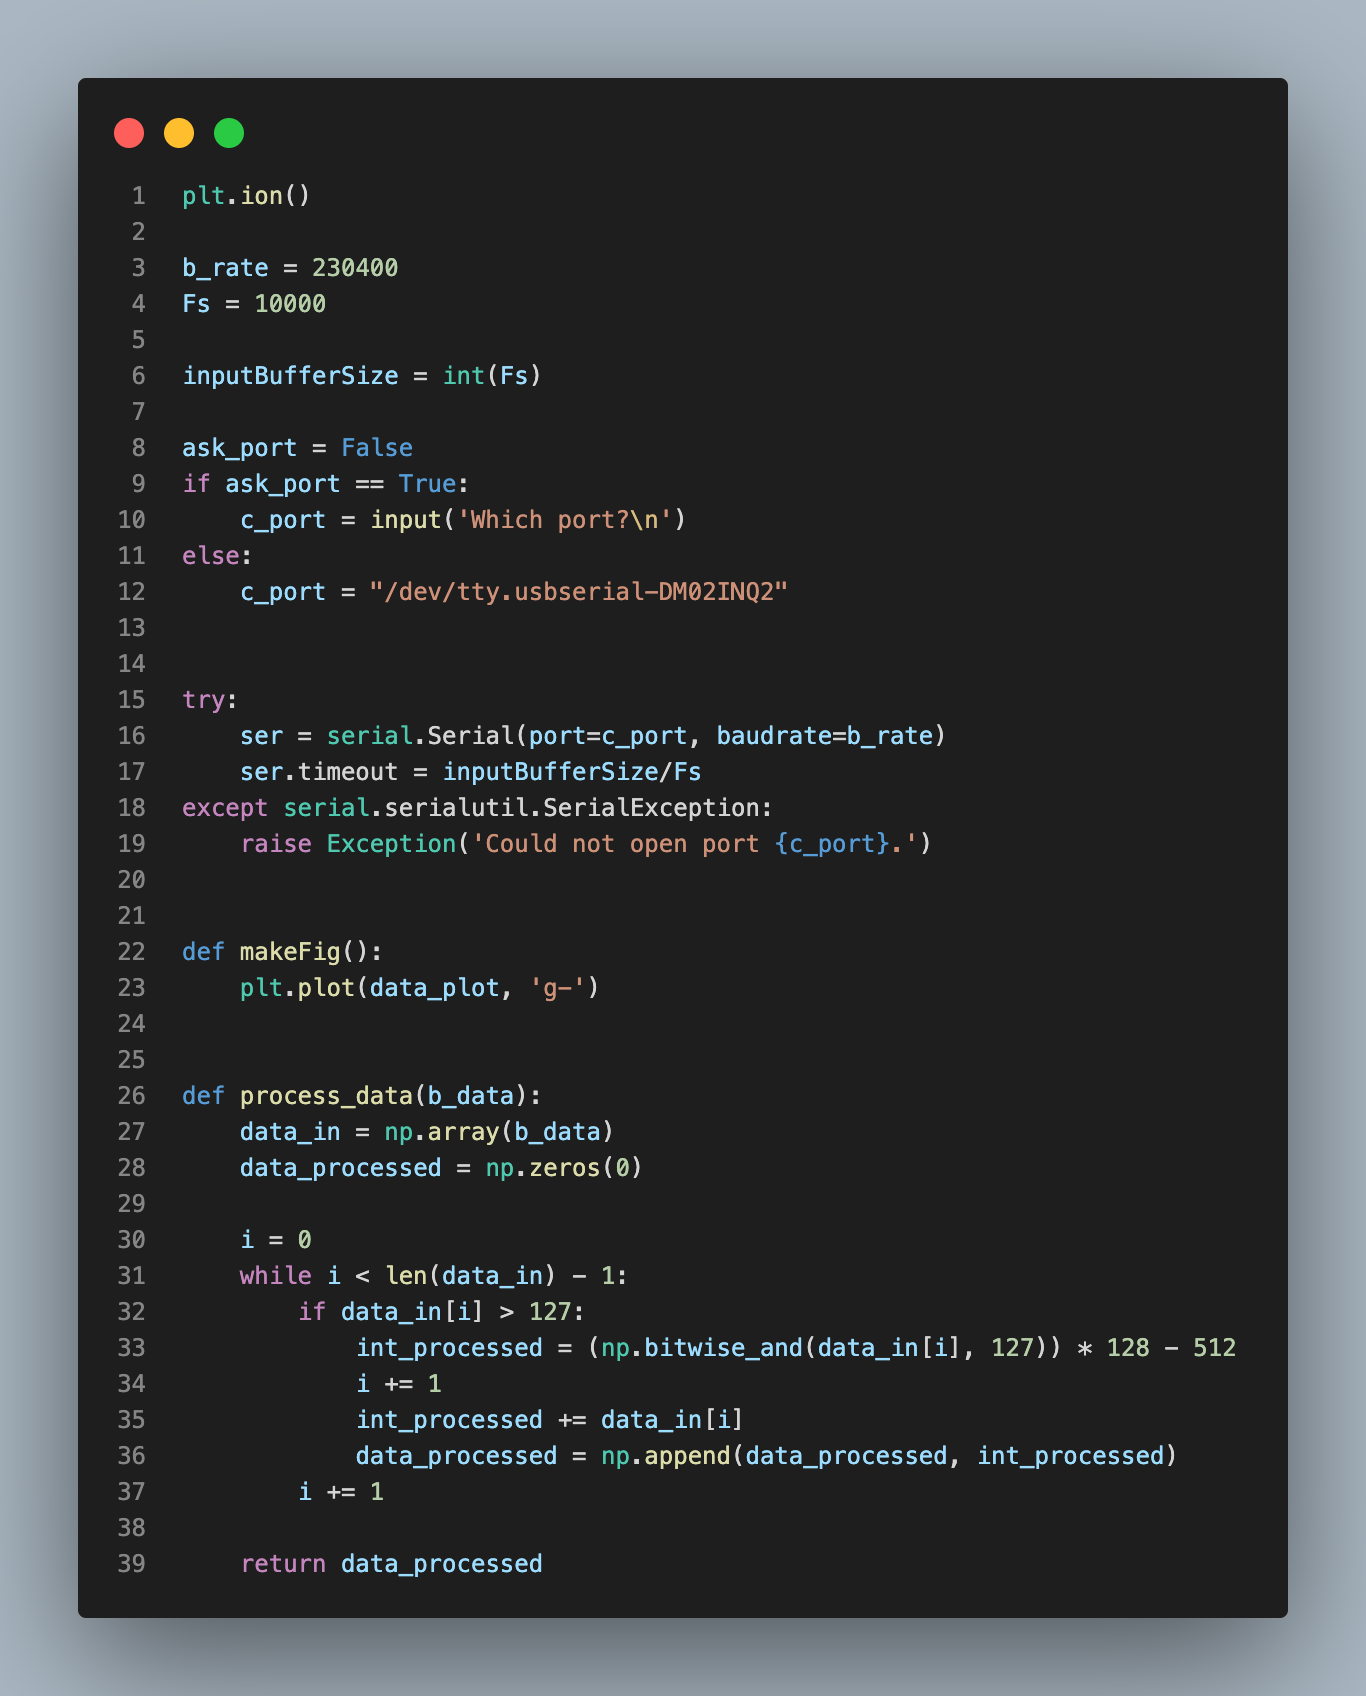
\includegraphics[width = 17cm, height = 15cm]{Pictures/arduino.png}
  \end{figure}
  
  
\newpage
\subsection{Part 2: Feature Extraction and Classifier Choice}

Code can be found in \href{https://github.com/yingzhenwang/Brain/blob/main/notebook.ipynb}{notebook.ipynb}

\begin{figure}[H]
  \centering
  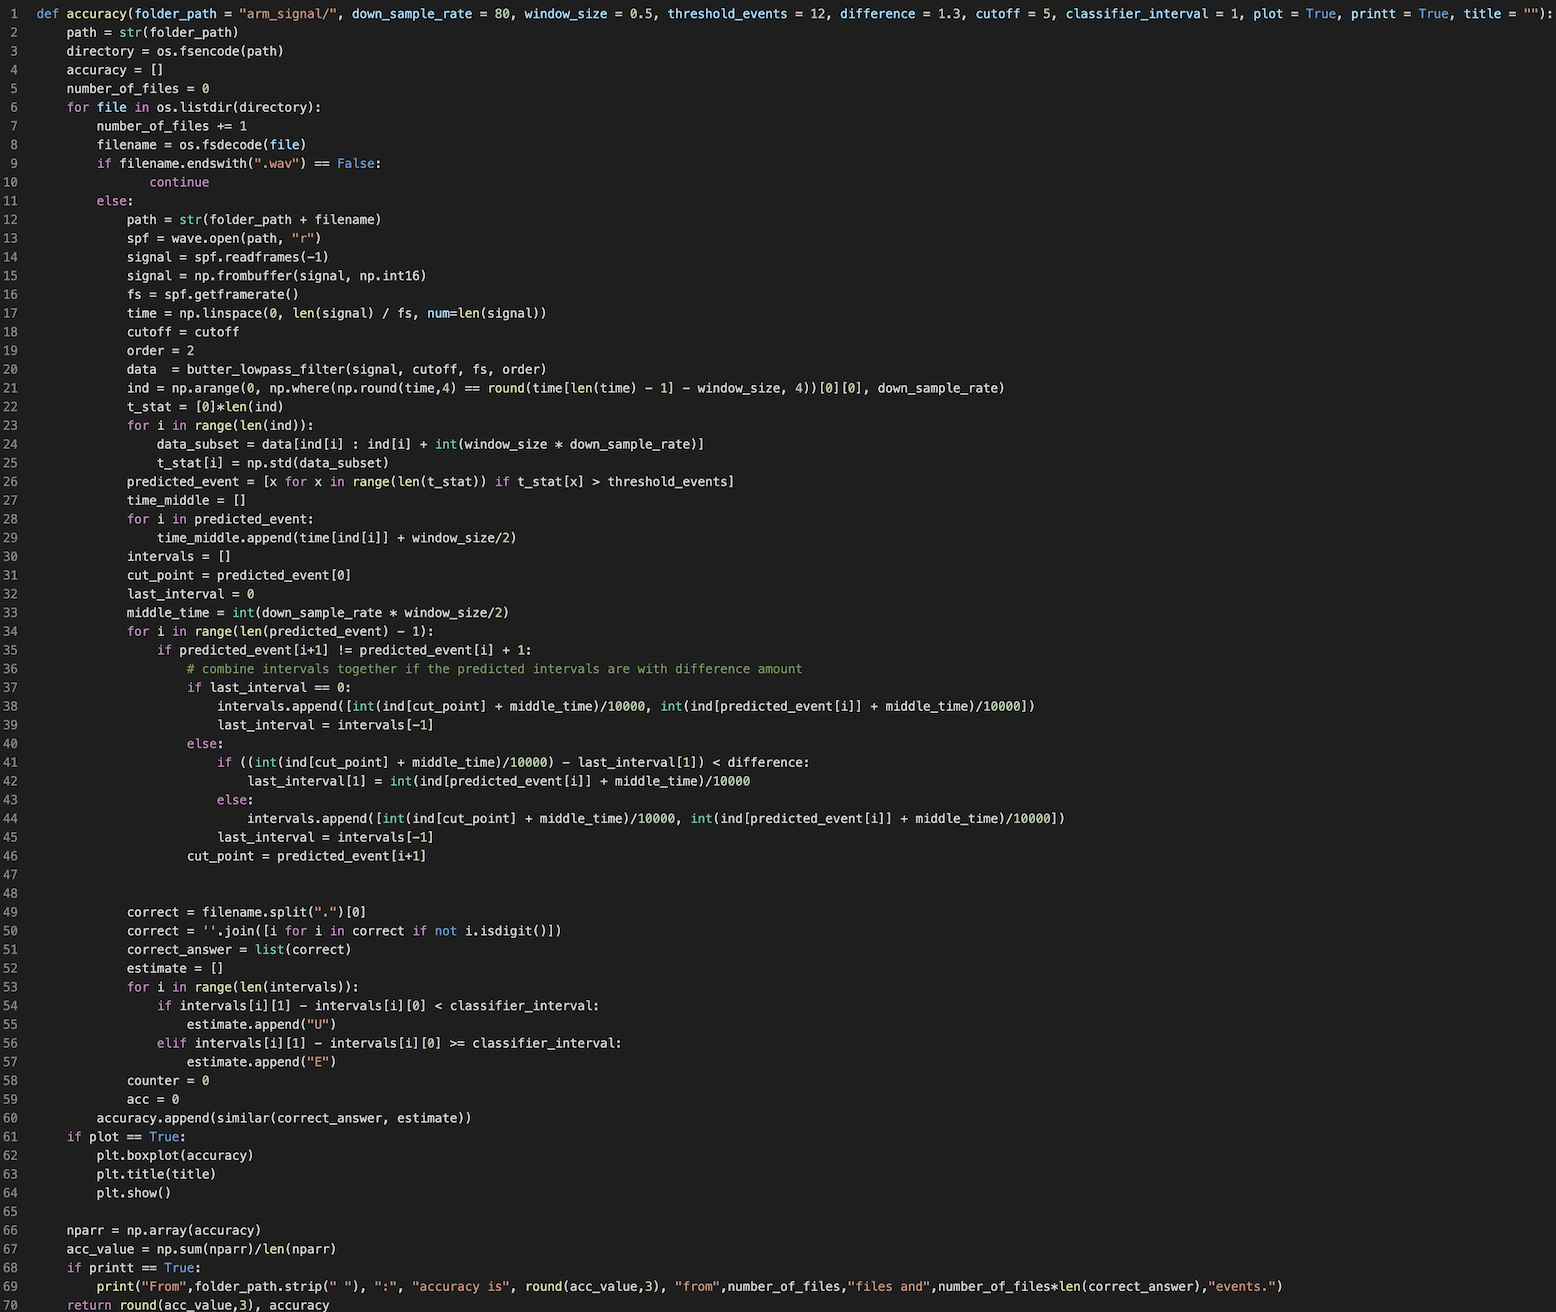
\includegraphics[width = 17cm, height = 18cm]{Pictures/acc_cut.png}
  \end{figure}

\newpage

\subsection{Part 3: Live Deployment}

The complete code can be found in \href{https://github.com/yingzhenwang/Brain/blob/main/Chrome/live.py}{Live.py}
\begin{figure}[H]
  \centering
  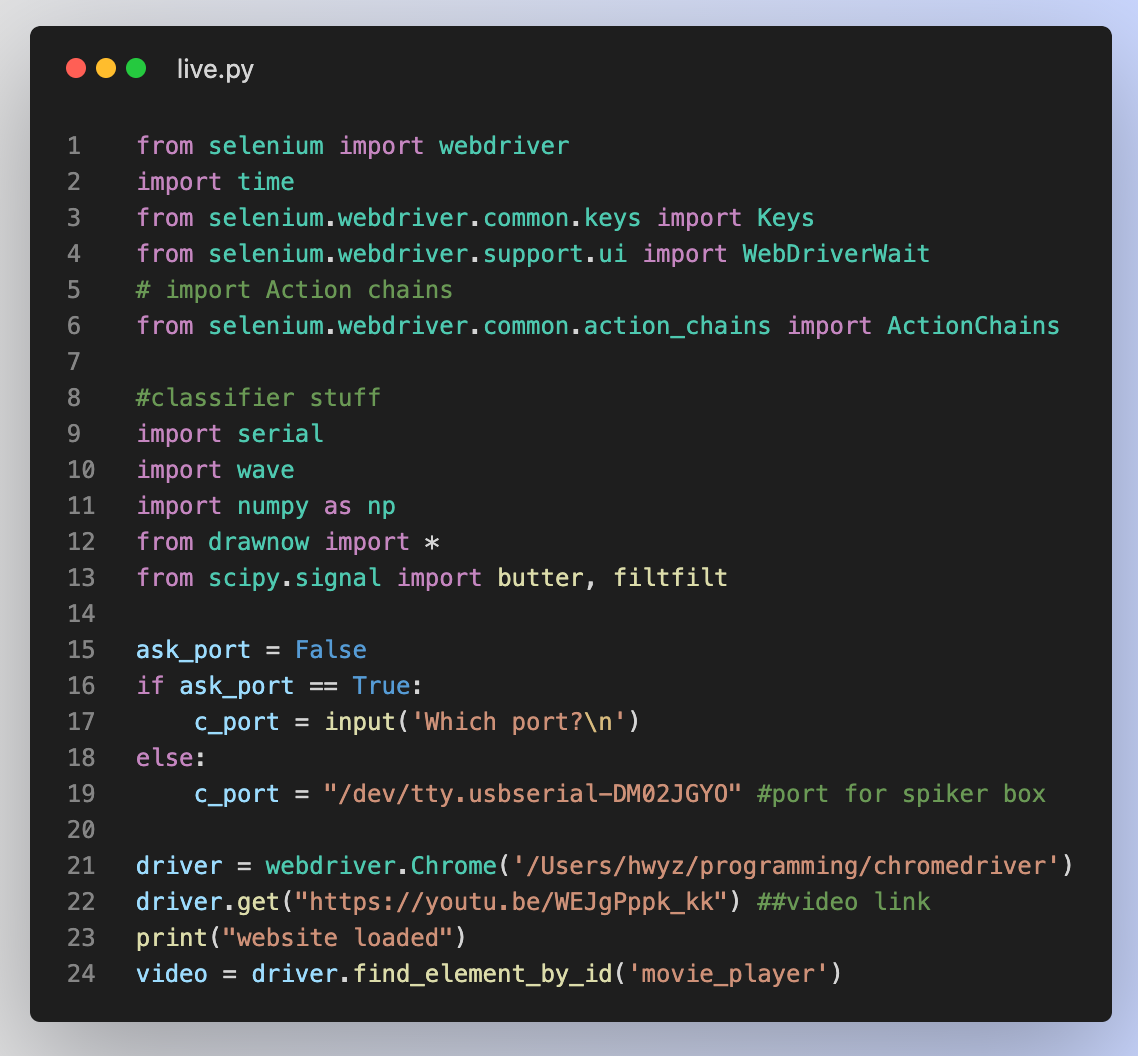
\includegraphics[width = 17cm, height = 18cm]{Pictures/live_2.png}
  \end{figure}


\newpage

\section{Student Contributions}
Group Members: 

Jamie Nicholas | SID: 490424858

Jamie's role included data collection, this requires testing of the placements of the electrodes and collecting different sequences of data from various parts of the body. Additionally, process documentation and report writing and editing. 

Yuxan Cheng | SID: 490062904

Yuxan's role included data collection, designing the arm movements, making observation of electric signals from arm movements, and performing the process of streaming.

Martin Huang | SID: 500494994

Martin's role included the primary organisation of Training data and Classification ruling. Martin designed the classification ruling for static wave files in order to determine a classification rule for interval prediction and event prediction. This classification rule configurations were tested with 672 unique modifications, and was used to connect the paths between data collection and live testing.

Harry Wang | SID: 490556311

Harry's role included the construction of the final live classifier we used, live classifier testing and parameter tuning of the live classifier. Harry is also in charge of the deployment of our product, which included writing the Selenium script for chrome automation and deployment testing.

\newpage
\section{References}

% BibTex
\nocite{*}
\bibliographystyle{alpha}
\bibliography{reference,packages}




Word Count: 2594
\end{document}